% Written by src/detection/final_figures.py; needs \usepackage{graphicx} and results/figures/ in \graphicspath.
\begin{figure*}[tb]
  \centering
  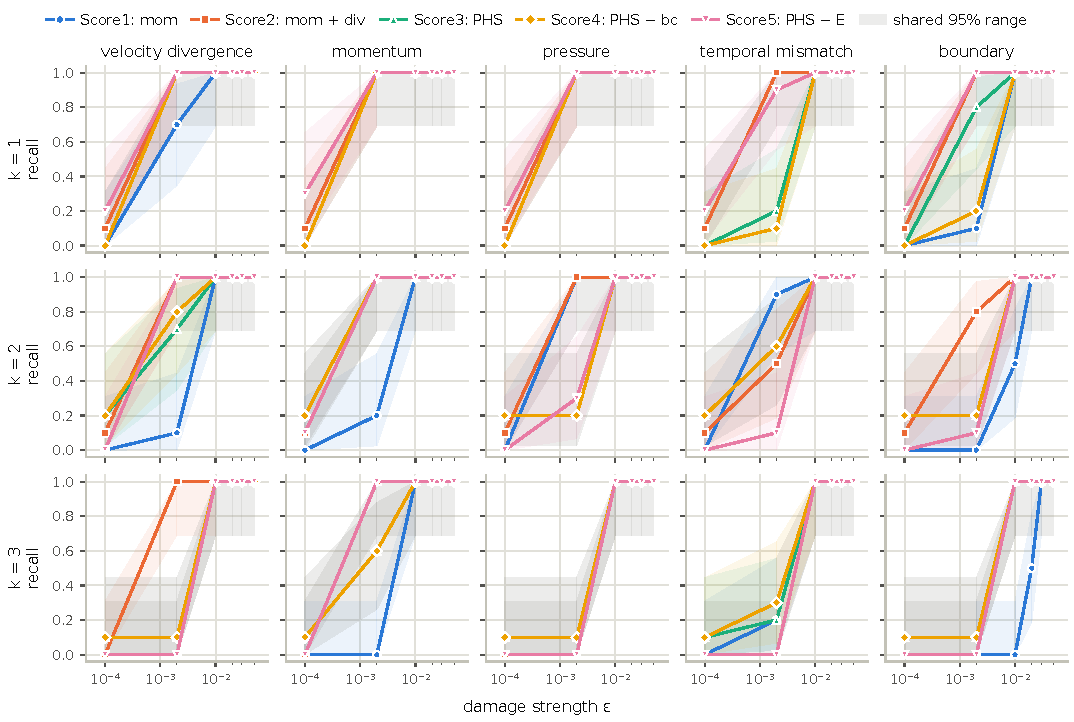
\includegraphics[width=\textwidth]{fig_recall_vs_eps_by_k.pdf}
  \caption{Recall as in Fig.~\ref{fig:recall_vs_eps}, split by $k$ (rows): each point is out of the 10 cases with that $k$, with exact 95\% confidence intervals (Table~\ref{tab:recall_by_type_eps_k}). Recall falls with $k$ for every score: at $\varepsilon = 0.002$, the damaged fields flagged out of 50 (5 types $\times$ 10 cases) for $k = 1, 2, 3$ are Score1 38, 22, 2; Score2 50, 43, 20; Score3 40, 27, 11; Score4 33, 28, 12; Score5 49, 25, 10. Pooled over the six strengths instead (Table~\ref{tab:benchmark_metrics_by_k}), some case-bootstrap confidence intervals have no width: Score2's recall for $k = 3$ is 0.733 [0.733, 0.733], because every $k = 3$ case has 22 of its 30 damaged fields flagged, so no resample of cases can change the rate (also Score5 for $k = 3$, 0.700 [0.700, 0.700], every case 21 of 30). The exact intervals per strength shown here don't have this problem.}
  \label{fig:recall_vs_eps_by_k}
\end{figure*}
